\documentclass[border=10pt,crop=true]{standalone}
\usepackage{tikz}

% 时间轴：0--20 ms；$x=0.3$ cm/ms
% 上：$v_i$ 阶跃 1 V；下：$v_o$ 在 13 ms 饱和于 $-13$ V

\begin{document}
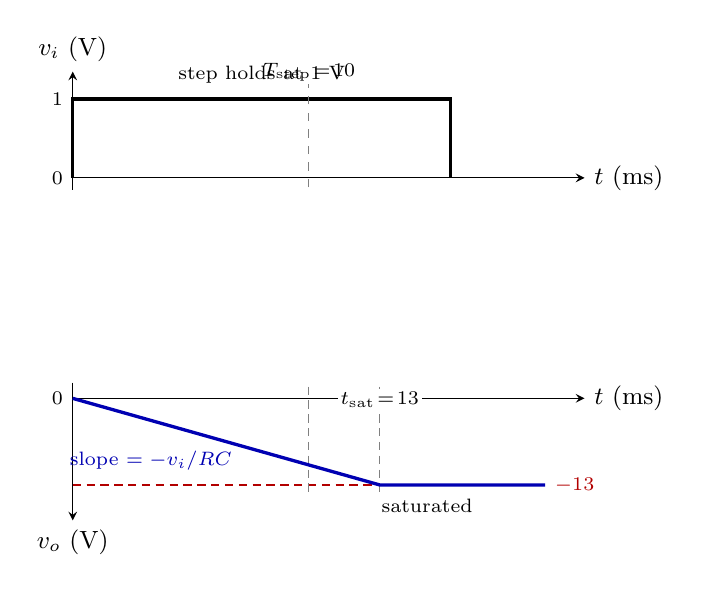
\begin{tikzpicture}[font=\small, >=stealth]
  \def\xms{0.30}     % cm per ms
  \def\Tend{20}
  \def\Tsat{13}
  \def\Trec{10}
  \def\Tstep{16}
  \def\ViH{1.0}      % V, top panel height (cm)
  \def\VoSat{1.10}   % cm for 13 V on bottom panel

  \pgfmathsetmacro{\Xend}{\Tend*\xms}
  \pgfmathsetmacro{\Xsat}{\Tsat*\xms}
  \pgfmathsetmacro{\Xrec}{\Trec*\xms}
  \pgfmathsetmacro{\Xstep}{\Tstep*\xms}

  % ----- $v_i$ -----
  \begin{scope}[shift={(0,2.8)}]
    \draw[->] (0,0) -- (\Xend+0.5,0) node[right] {$t$ (ms)};
    \draw[->] (0,-0.15) -- (0,\ViH+0.35) node[above] {$v_i$ (V)};
    \node[left, font=\scriptsize] at (0,0) {$0$};
    \node[left, font=\scriptsize] at (0,\ViH) {$1$};
    \draw[very thick] (0,0) -- (0,\ViH) -- (\Xstep,\ViH) -- (\Xstep,0);
    \draw[dashed, gray] (\Xrec,-0.12) -- (\Xrec,\ViH+0.2);
    \node[font=\scriptsize, fill=white, inner sep=1pt, anchor=south]
      at (\Xrec,\ViH+0.18) {$T_{\mathrm{step}}\!=\!10$};
    \node[font=\scriptsize, anchor=south] at (0.5*\Xstep,\ViH+0.08)
      {step holds at $1$ V};
  \end{scope}

  % ----- $v_o$ -----
  \begin{scope}
    \draw[->] (0,0) -- (\Xend+0.5,0) node[right] {$t$ (ms)};
    \draw[->] (0,0.2) -- (0,-\VoSat-0.45) node[below] {$v_o$ (V)};
    \node[left, font=\scriptsize] at (0,0) {$0$};
    \draw[densely dashed, red!70!black] (0,-\VoSat) -- (\Xend,-\VoSat);
    \node[right, font=\scriptsize, red!70!black] at (\Xend,-\VoSat) {$-13$};
    \draw[densely dashed, gray] (\Xsat,0.15) -- (\Xsat,-\VoSat-0.15);
    \node[font=\scriptsize, fill=white, inner sep=1pt, anchor=north]
      at (\Xsat,0.12) {$t_{\mathrm{sat}}\!=\!13$};
    \draw[densely dashed, gray] (\Xrec,0.15) -- (\Xrec,-\VoSat-0.15);
    \draw[very thick, blue!70!black] (0,0) -- (\Xsat,-\VoSat) -- (\Xend,-\VoSat);
    \node[font=\scriptsize, blue!70!black, anchor=north east]
      at (0.55*\Xsat,-0.5*\VoSat) {slope $=-v_i/RC$};
    \node[font=\scriptsize, anchor=north] at (0.75*\Xend,-\VoSat-0.06)
      {saturated};
  \end{scope}
\end{tikzpicture}
\end{document}
